\documentclass[a4paper]{article}
% Some basic packages
\usepackage{graphicx}

% Don't indent paragraphs, leave some space between them
\usepackage{parskip}

% Hide page number when page is empty
\usepackage{emptypage}
\usepackage{subcaption}
\usepackage{multicol}
\usepackage{xcolor}


% Math stuff
\usepackage{amsmath, amsfonts, mathtools, amsthm, amssymb}
% Fancy script capitals
\usepackage{mathrsfs}
\usepackage{cancel}
% Bold math
\usepackage{bm}
% Some shortcuts
\newcommand\N{\ensuremath{\mathbb{N}}}
\newcommand\R{\ensuremath{\mathbb{R}}}
\newcommand\Z{\ensuremath{\mathbb{Z}}}
\renewcommand\O{\ensuremath{\emptyset}}
\newcommand\Q{\ensuremath{\mathbb{Q}}}
\newcommand\C{\ensuremath{\mathbb{C}}}

% Easily typeset systems of equations (French package)
\usepackage{systeme}

% Put x \to \infty below \lim
\let\svlim\lim\def\lim{\svlim\limits}

%Make implies and impliedby shorter
\let\implies\Rightarrow
\let\impliedby\Leftarrow
\let\iff\Leftrightarrow
\let\epsilon\varepsilon


% horizontal rule
\newcommand\hr{
    \noindent\rule[0.5ex]{\linewidth}{0.5pt}
}

% hide parts
\newcommand\hide[1]{}

% si unitx
\usepackage{siunitx}

% Environments
\makeatother
% For box around Definition, Theorem, \ldots
\usepackage{mdframed}
\mdfsetup{skipabove=1em,skipbelow=0em}
\theoremstyle{definition}
\newmdtheoremenv[nobreak=true]{definitie}{Definitie}
\newmdtheoremenv[nobreak=true]{eigenschap}{Eigenschap}
\newmdtheoremenv[nobreak=true]{gevolg}{Gevolg}
\newmdtheoremenv[nobreak=true]{lemma}{Lemma}
\newmdtheoremenv[nobreak=true]{propositie}{Propositie}
\newmdtheoremenv[nobreak=true]{stelling}{Stelling}
\newmdtheoremenv[nobreak=true]{wet}{Wet}
\newmdtheoremenv[nobreak=true]{postulaat}{Postulaat}
\newmdtheoremenv{conclusie}{Conclusie}
\newmdtheoremenv{toemaatje}{Toemaatje}
\newmdtheoremenv{vermoeden}{Vermoeden}
\newtheorem*{herhaling}{Herhaling}
\newtheorem*{intermezzo}{Intermezzo}
\newtheorem*{notatie}{Notatie}
\newtheorem*{observatie}{Observatie}
\newtheorem*{oef}{Oefening}
\newtheorem*{opmerking}{Opmerking}
\newtheorem*{praktisch}{Praktisch}
\newtheorem*{probleem}{Probleem}
\newtheorem*{terminologie}{Terminologie}
\newtheorem*{toepassing}{Toepassing}
\newtheorem*{uovt}{UOVT}
\newtheorem*{vb}{Voorbeeld}
\newtheorem*{vraag}{Vraag}

\newmdtheoremenv[nobreak=true]{definition}{Definition}
\newtheorem*{eg}{Example}
\newtheorem*{notation}{Notation}
\newtheorem*{previouslyseen}{As previously seen}
\newtheorem*{remark}{Remark}
\newtheorem*{note}{Note}
\newtheorem*{problem}{Problem}
\newtheorem*{observe}{Observe}
\newtheorem*{property}{Property}
\newtheorem*{intuition}{Intuition}
\newmdtheoremenv[nobreak=true]{prop}{Proposition}
\newmdtheoremenv[nobreak=true]{theorem}{Theorem}
\newmdtheoremenv[nobreak=true]{corollary}{Corollary}

% End example and intermezzo environments with a small diamond (just like proof
% environments end with a small square)
\usepackage{etoolbox}
\AtEndEnvironment{vb}{\null\hfill$\diamond$}%
\AtEndEnvironment{intermezzo}{\null\hfill$\diamond$}%
% \AtEndEnvironment{opmerking}{\null\hfill$\diamond$}%

% Fix some spacing
% http://tex.stackexchange.com/questions/22119/how-can-i-change-the-spacing-before-theorems-with-amsthm
\makeatletter
\def\thm@space@setup{%
  \thm@preskip=\parskip \thm@postskip=0pt
}


% Exercise 
% Usage:
% \oefening{5}
% \suboefening{1}
% \suboefening{2}
% \suboefening{3}
% gives
% Oefening 5
%   Oefening 5.1
%   Oefening 5.2
%   Oefening 5.3
\newcommand{\oefening}[1]{%
    \def\@oefening{#1}%
    \subsection*{Oefening #1}
}

\newcommand{\suboefening}[1]{%
    \subsubsection*{Oefening \@oefening.#1}
}


% \lecture starts a new lecture (les in dutch)
%
% Usage:
% \lecture{1}{di 12 feb 2019 16:00}{Inleiding}
%
% This adds a section heading with the number / title of the lecture and a
% margin paragraph with the date.

% I use \dateparts here to hide the year (2019). This way, I can easily parse
% the date of each lecture unambiguously while still having a human-friendly
% short format printed to the pdf.

\usepackage{xifthen}
\def\testdateparts#1{\dateparts#1\relax}
\def\dateparts#1 #2 #3 #4 #5\relax{
    \marginpar{\small\textsf{\mbox{#1 #2 #3 #5}}}
}

\def\@lecture{}%
\newcommand{\lecture}[3]{
    \ifthenelse{\isempty{#3}}{%
        \def\@lecture{Lecture #1}%
    }{%
        \def\@lecture{Lecture #1: #3}%
    }%
    \subsection*{\@lecture}
    \marginpar{\small\textsf{\mbox{#2}}}
}



% These are the fancy headers
\usepackage{fancyhdr}
\pagestyle{fancy}

% LE: left even
% RO: right odd
% CE, CO: center even, center odd
% My name for when I print my lecture notes to use for an open book exam.
% \fancyhead[LE,RO]{Gilles Castel}

% \fancyhead[RO,LE]{\@lecture} % Right odd,  Left even
% \fancyhead[RE,LO]{}          % Right even, Left odd

% \fancyfoot[RO,LE]{\thepage}  % Right odd,  Left even
% \fancyfoot[RE,LO]{}          % Right even, Left odd
\fancyfoot[C]{\leftmark}     % Center

\makeatother




% Todonotes and inline notes in fancy boxes
\usepackage{todonotes}
\usepackage{tcolorbox}

% Make boxes breakable
\tcbuselibrary{breakable}

% Verbetering is correction in Dutch
% Usage: 
% \begin{verbetering}
%     Lorem ipsum dolor sit amet, consetetur sadipscing elitr, sed diam nonumy eirmod
%     tempor invidunt ut labore et dolore magna aliquyam erat, sed diam voluptua. At
%     vero eos et accusam et justo duo dolores et ea rebum. Stet clita kasd gubergren,
%     no sea takimata sanctus est Lorem ipsum dolor sit amet.
% \end{verbetering}
\newenvironment{verbetering}{\begin{tcolorbox}[
    arc=0mm,
    colback=white,
    colframe=green!60!black,
    title=Opmerking,
    fonttitle=\sffamily,
    breakable
]}{\end{tcolorbox}}

% Noot is note in Dutch. Same as 'verbetering' but color of box is different
\newenvironment{noot}[1]{\begin{tcolorbox}[
    arc=0mm,
    colback=white,
    colframe=white!60!black,
    title=#1,
    fonttitle=\sffamily,
    breakable
]}{\end{tcolorbox}}




% Figure support as explained in my blog post.
\usepackage{import}
\usepackage{xifthen}
% \pdfminorversion=7
\usepackage{pdfpages}
\usepackage{transparent}
\newcommand{\incfig}[1]{%
    \def\svgwidth{\columnwidth}
    \import{./figures/}{#1.pdf_tex}
}

% Fix some stuff
% %http://tex.stackexchange.com/questions/76273/multiple-pdfs-with-page-group-included-in-a-single-page-warning
\pdfsuppresswarningpagegroup=1


% My name
\author{S. Bettani}


\DeclareMathOperator{\length}{length}
\DeclareMathOperator{\Aut}{Aut}
\DeclareMathOperator{\diam}{diam}
\DeclareMathOperator*{\res}{res}

\title{Psicopatologia}

\begin{document}
    \maketitle
    \tableofcontents
    % start lectures
    \lecture{1}{Sun 08 Mar 2020 19:15}{Introduzione}{
Quali sono gli elementi che distinguono nell'\textbf{immaginario comune} la normalità?

\begin{enumerate}
	\item Compromissione di competenze
	\item Ricerca di aiuto
	\item Sofferenza
	\item Irrazionalità 
	\item Trasgressione 
	\item Devianza statistica
\end{enumerate}

In realtà pochi di questi criteri funziona, come il \textbf{dolore}, ma non sempre: a volte i pazienti si sentono estremamente bene (mania, ipomania, psicopatia), e a volte persone non malate soffrono.

Anche la compromissione o disabilità funziona come principio diagnostico, ed è il più utilizzato nei manuali diagnostici, ma ha dei limiti: condizioni rare possono essere vantaggiose, alcune condizioni non sono misurabili e alcune patologie possono essere normali nella società contemporanea.

\paragraph{Esempio Clinico}  

Cinzia: ragazza normale di 21 anni, ad una certa smette di uscire e di andare bene a scuola, e sta chiusa in casa tutto il giorno.

Il processo diagnostico consiste nella verifica di \textbf{ipotesi}, fermarsi troppo presto nel processo è molto rischioso
\medskip\\

\includegraphics[width=\linewidth]{./images/image1}
\medskip\\

I criteri: la presenza di più fattori è necessaria, assieme al loro covariare nel tempo.
Anche un solo episodio depressivo è sufficiente per dire che una persone ha un disturbo mentale.
Gli stessi comportamenti hanno diversi significati a diverse età.
Il contesto a volte spiega il comportamento meglio di una malattia.
Anche i fattori culturali devono essere considerati, ogni cultura ha modalità di reazione al lutto considerate normali.



    \lecture{2}{Mon 09 Mar 2020 13:41}{Definizione e Classificazione}{

\begin{itemize}
	\item Segni: indicatori di malattia osservabili
	\item Sintomi: percezione soggettiva di malessere
	\item Sindrome: covariazione di sintomi/segni, eziologia non nota
	\item Malattia: sindrome con eziologia, prognosi e decorso noti e caratteristici
\end{itemize}

In psicopatologia le l'eziologia è sempre multi fattoriale.
\medskip\\
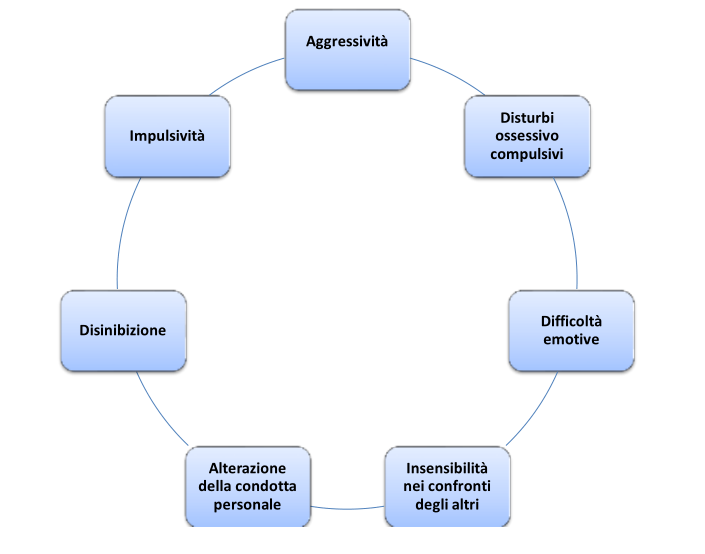
\includegraphics[width=\linewidth]{./images/image2}
\medskip\\

Secondo la visione biopsicosociale ci sono fattori:

\begin{itemize}
	\item Predisponenti
	\item Precipitanti
	\item Perpetuanti (di mantenimento) 
	\item Protettivi
\end{itemize} 
\begin{quote}
	\emph{ “La malattia mentale potrebbe (o dovrebbe) essere definita solo in presenza di dati quali: un’eziologia accertata (conoscenza delle cause e dei fattori che favoriscono o inibiscono il processo morboso); corrispondenti reperti anatomo-biologici; e rilievi patogenetici (correlazioni dimostrabili tra cause, reperti biologici ed effetti sintomatologici obiettivabili)”. }
	\begin{flushright}
		Gilberti et al., 1996
	\end{flushright}
\end{quote}

In realtà non abbiamo informazioni sulla malattia:
\medskip\\

\includegraphics[width=\linewidth]{./images/image1}
\medskip\\
Ovviamente la diagnosi non è altro che un'etichetta, un nome comune, come \emph{giraffa}, che ci dà però informazioni molto precise.

La definizione del DSM-5 del disturbo mentale è: 
\medskip\\

\includegraphics[width=\linewidth]{./images/image3}
\medskip\\
Un disturbo mentale è una sindrome caratterizzata da un’alterazione clinicamente significativa della sfera cognitiva, della regolazione delle emozioni o del comportamento di un individuo, che riflette una disfunzione nei processi psicologici, biologici o evolutivi che sottendono il funzionamento mentale.

    \documentclass[12pt, a4paper]{article}
\usepackage{graphicx}

\date{8 Gennaio 2020}
\title{None}
\author{myyuni}

\begin{document}

\maketitle

\section{}


















\end{document}

    \lecture{4}{Tue 10 Mar 2020 14:32}{La Psicopatologia Generale}{

Nel corso del tempo sono più che triplicate le diverse categorizzazioni di disturbi mentali nei DSM.

L'introduzione del DSM ha contribuito a migliorare l'\textbf{attendibilità} della diagnosi (due psichiatri diagnosticano la stessa malattia) ma la validità non è migliorata (es. Rosenhan)

Per \textbf{psicopatologia} si può intendere la psicopatologia descrittiva o interpretativa.

\paragraph{ La Psicopatologia descrittiva} si occupa dello studio e della classificazione degli elementi invarianti dei disturbi mentali, procedendo per le grandi aree dello sviluppo psicologico (percettivo, dello sviluppo, etc.), inglobando la psicopatologia \emph{oggettiva e soggettiva} 

\paragraph{La Psicopatologia oggettiva} ha come ambito d'indagine la sola realtà esterna, ed è eredità di Kraeplin, e nasce come contrapposizione all'approccio soggettivo.

\paragraph{La Psicopatologia soggettiva} ha come obiettivo la valorizzazione delle esperienze soggettive, rifiuta i metodi delle scienze naturali, fondato da Jasper. Per spiegare gli eventi interni bisogna entrare nella prospettiva empatica.

\paragraph{Il limite della comprensibilità} è raggiunto quando non sono più possibili altro che spiegazioni causali, bisogna quindi spostarsi dalla comprensione alla spiegazione.  

\paragraph{Primario/Secondario} Nel dominio della spiegazione: primario si riferisce alla causa immediata, mentre secondario si intende l'effetto. Nel dominio della comprensione primario significa inderivabile, mentre secondario ciò che emerge dal primario.

\paragraph{Variabili importanti} 
\begin{itemize}
	\item Obiettivi dell'intervento: possono essere specifici o generali
	\item Il setting 
	\item Il contratto terapeutico.
	\item Valutazione clinica
	\item Importanza attribuita alla relazione
	\item Tecniche e procedure
\end{itemize}



    \documentclass[12pt, a4paper]{article}
\usepackage{graphicx}

\date{8 Gennaio 2020}
\title{None}
\author{myyuni}

\begin{document}

\maketitle

\section{<esc>:VimtexCompile<CR>}


















\end{document}

    \documentclass[12pt, a4paper]{article}
\usepackage{graphicx}

\date{8 Gennaio 2020}
\title{None}
\author{myyuni}

\begin{document}

\maketitle

\section{<C-[>:VimtexCompile}


















\end{document}

    \lecture{7}{Tue 17 Mar 2020 14:24}{Disturbi del pensiero}{

Possono essere di \textbf{forma} o \textbf{contenuto}  
\begin{itemize}
	\item Nei disturbi di forma ci sono problemi di ragionamento e a volte anche nel contenuto
	\item Nei disturbi di contenuto il problema sta solo nell'oggetto del pensiero, non nella modalità.
\end{itemize}
\paragraph{La diagnosi} avviene grazie alla comunicazione.  

\section{Disturbi della forma del pensiero} 
\paragraph{Caratteristiche}  
\begin{itemize}
	\item Alterazione della velocità
	\item Disorganizzazione
	\item Assenza di un'idea centrale
	\item Nessi causali distorti
	\item Incapacità di comprendere significati
\end{itemize}
\paragraph{I disturbi:}  
\begin{enumerate}
	\item Accelerazione: vengono prodotte troppe idee, viene compromessa l'efficacia della comunicazione ma i nessi causali sono conservati. Elevata distraibilità, pressione interna a parlare, la sovrapproduzione di idee viene percepita internamente come alta prestazione
	\item Fuga delle idee: forma estrema di accelerazione, la persona si distrae facilmente guidata da criteri come assonanza, somiglianza, rima, fattori casuali, \emph{tipica della mania} 
	\item Rallentamento: lentezza, bassa produttività, ridotta efficacia comunicativa. \emph{Tipica della depressione}, sensazione di fatica nel passare da un concetto all'altro, difficoltà nel prendere decisioni, mancanza di concentrazione, memoria e chiarezza. Il paziente può sviluppare un'\emph{idea sovrastimata} o \emph{delirante} che i pensieri gli sfuggano dalla mente.
	\item Ridondanza procedurale: abbondare di concetti, premesse infinite
	\item Perseverazione: non riesce a modificare il comportamento in base al feedback, pessimo punteggio nel Winsconsin Card Sorting Test.
	\item Tangenzialità: non si riesce ad andare nel cuore della comunicazione
	\item Illogicità: gravità estrema, non si arriva alle conclusioni logiche, i nessi sono insensati.
	\item Distraibilità
	\item Associazioni per assonanza
	\item Neologismo
\end{enumerate}
\paragraph{I disturbi estremi}  
\begin{itemize}
	\item Blocco del pensiero: arresto non intenzionale dell'eloquio e presumibilmente del pensiero, percezione soggettiva che il pensiero si blocchi, spiegazione del paziente come \emph{sottrazione del pensiero}. Associato alla \emph{schizofrenia}. 
	\item Concretismo: ridotta o assente capacità di operare astrazioni, può apparire in \emph{deficit intellettivi} o \emph{demenza} 
\end{itemize}
\section{Disturbi del contenuto del pensiero}
\paragraph{I disturbi}  
\begin{itemize}
	\item Delirio: sempre un fenomeno patologico, indice di follia, ci sono 3 criteri definitori:
		\begin{enumerate}
			\item Impossibilità del contenuto, criterio confondente, non solo i deliri bizzarri sono deliranti.
			\item Certezza impareggiabile della veridicità dell'idea, come per dogmi religiosi, filosofici o scientifici.
			\item Incorreggibilità, immodificabilità, non è necessariamente patologica, ma c'è differenza tra certezza patologica e non.
		\end{enumerate}

	\item Idea prevalente: non necessariamente patologica
	\item (Ossessione)
\end{itemize}


    \lecture{8}{Thu 19 Mar 2020 09:08}{Deliri}{

\paragraph{Il criterio dell'impossibilità} nel delirio non viene citata nel DSM V.
Il problema non sta nella plausibilità dell'idea, ma del modo in cui ci arriva, nelle prove che porta e nei comportamenti che produce.

\paragraph{La struttura auto-centrica}  è quasi sempre presente, tutto ha significato per il paziente. Per esempio il paziente:
\begin{itemize}
	\item è oggetto di persecuzioni
	\item è destinatario di messaggi allusivi
	\item è colui a cui le voci si rivolgono
	\item è responsabile di tutti i mali
	\item è colui a cui viene sottratto il pensiero 
	\item impersonifica la divinità 
	\item acquisisce capacità o poteri
\end{itemize}
\paragraph{Forma e contenuto}  del delirio: La forma ci permette di eliminare alcune possibilità di diagnosi e di evidenziarne altre, ma anche il contenuto può informare sul tipo di patologia. Ad esempio se i temi di colpa, rovina e morti sono presenti nel delirio, andremo a cercare un disturbo depressivo, mentre in caso di un quadro di eccitamento maniacale ci aspetteremmo deliri con contenuti di grandiosità.

Questo ci è utile per trovare congruenze o incongruenze tra l'umore dominante e i contenuti deliranti.

\paragraph{Idee simil-deliranti}
Presenti in disturbi dell'umore
\medskip\\
\includegraphics[width=\linewidth]{./images/image9}
\medskip\\
\paragraph{Deliri veri o primari} presenti in patologie 
\medskip\\
\includegraphics[width=\linewidth]{./images/image10}
\medskip\\
\section{Classificazione dei deliri per contenuto}
\begin{itemize}
	\item Persecuzione
	\item Riferimento
	\item Colpa
	\item Negazione
	\item Grandezza
	\item Erotico
	\item Ipocondriaco
	\item Mistico
\end{itemize}

\paragraph{Il delirio di persecuzione}  è estremamente frequente, si trova in schizofrenia, nella mania in disturbi deliranti. Consiste nel fatto che il paziente:
\begin{itemize}
	\item Si sente oggetto di attenzione \emph{ostile} da parte di altre persone
	\item Si sente osservato, spiato, seguito o controllato
	\item Teme di essere drogato o avvelenato (delirio di veneficio)
	\item È convinto di complotti ai suoi danni
	\item Vede fatti, gesti o oggetti come dotati di significato ostile
\end{itemize}
\paragraph{Il delirio di riferimento}  è la convinzione che situazioni, oggetti, persone, fatti assumano un particolare significato allusivo riferito alla propria persona. Quasi sempre i contenuti sono a connotazione ostile, ma \emph{manca un contenuto persecutorio chiaramente espresso}. È frequente nella schizofrenia.

\paragraph{Deliri di colpa}  o di indegnità o rovina. Il paziente:
\begin{itemize}
	\item Si sente responsabile di danni e sciagure
	\item Si sente rovinato, distrutto indegno, di essere umano
	\item Pensa di aver condotto se stesso e le persone vicine a lui alla rovina economica e sociale
	\item È convinto che continuare a vivere significhi perpetuare in eterno questa condizione
\end{itemize}
C'è rischio di suicidio o di omicidio-suicidio.

\paragraph{Delirio di negazione}  o nichilistico. Piuttosto raro, si può trovare in disturbi depressivi o nella schizofrenia. Consiste nella convinzione della non esistenza di sé, o di una parte di sé.

\paragraph{Delirio di grandezza} contenuto speculare a quello di colpa, indegnità o rovina, accompagna spesso la mania. Il paziente si può sentire ricco potente, eccetera.

\paragraph{Delirio erotico}  piuttosto raro, maggiore prevalenza nel sesso femminile, la paziente può essere convinta di possedere un'attrattività erotica fuori dal comune, di essere oggetto di corteggiamenti e di essere in grado di effettuare ogni tipo di conquista sessuale.

\paragraph{Delirio di gelosia}  Prevalente nel sesso maschile dopo i 40 anni, spesso associato all'alcolismo. Convinzione dell'infedeltà sopratutto a livello sessuale del partner. Non centrato su un'unica persona, ma su molteplici relazioni. Può essere difficile classificarlo come delirio.

\paragraph{Delirio mistico}  Il punto critico è legato alla caratteristica auto-centrica. Il paziente può riferire di comunicare direttamente con Dio, esserne messaggero ecc.

\paragraph{Delirio ipocondriaco} Convinzione di soffrire di una malattia fisica in assenza di qualsiasi rilievo obiettivo. È piuttosto comune, può fare comparsa anche nei disturbi dell'umore depressivi, negli anziani, mentre nei giovani è spesso in rapporto a fattori organici come traumi cranici o abuso di sostanze.

\paragraph{Deliri bizzarri}  sono chiaramente non plausibili e non comprensibili.

\paragraph{Deliri di influenzamento}  tema del controllo, il paziente si sente trasformata in un automa in balia di forze esterne e minacciose, abbinate a disturbi della forma.
\begin{itemize}
	\item Inserimento del pensiero, il paziente sa che alcuni contenuti della sua coscienza non gli appartengono
\item Furto del pensiero, il paziente percepisce il suo pensiero come asportato o rubato, associato a \emph{blocco del pensiero}
	\item Trasmissione del pensiero, il paziente sente che la sua attività di pensiero, le sue emozioni ricordi e desideri non sono più privati ma diffusi e conosciuti pubblicamente.
\end{itemize}

\paragraph{Sintomi di primo rango} Indicano la presenza di schizofrenia. 
\begin{itemize}
	\item Si devono presentare frequentemente nella schizofrenia
	\item Non devono verificarsi in condizioni diverse dalla schizofrenia
	\item Non dev'essere ambiguo identificare il sintomo
\end{itemize}
E sono:
\begin{itemize}
	\item Esperienze dispercettive, voci dialoganti, eco del pensiero.
	\item Passività del pensiero, inserzione, sottrazione e diffusione del pensiero.
	\item Percezioni deliranti, percezione normale interpretata dal paziente in modo delirante e considerata molto significativa.
	\item Esperienze di passività più generali, nell'ambito dell'affettività, del corpo, della volontà.
\end{itemize}

\paragraph{Disturbi del pensiero non deliranti}  
\begin{itemize}
	\item Le ossessioni: non è un'idea (o impulso o immagine) strana o assurda, ma è patologica per quanto la persona la considera rilevante, per la sua persistenza e ricorrenza. Implicano ansia e senso di colpa nel soggetto. I pensieri sono particolarmente ripugnanti per l'individuo, per esempio persone religiose possono essere tormentate da pensieri blasfemi. Il paziente appaiono contro la volontà del paziente, che attua una resistenza. Per questo le allucinazioni non possono essere ossessivi
	\item Le idee prevalenti: non sono false e incorreggibili, non sono percepite prive di senso, quindi non c'è resistenza dall'individuo, al contrario. Sono simili a convinzioni politiche, etiche o religiose radicali. Possono essere associate a personalità abnormi, e ad un'intensa componente affettiva. Contenuti frequenti:
		\begin{itemize}
			\item Idee persecutorie (tipo querulomane o religioso)
			\item Gelosia
			\item Ipocondria
			\item Dismorfofobia
			\item Parassitofobia
			\item Anoressia
			\item Innamoramento
		\end{itemize}
\end{itemize}
\includegraphics[width=\linewidth]{./images/image14}

    \lecture{9}{Mon 23 Mar 2020 10:05}{Disturbi dell'umore}{

Dobbiamo distinguere tra:
\begin{itemize}
	\item Umore: stato affettivo di base di un individuo, prevalente e prolungato o disposizionale.
	\item Emozione: esperienza spontanea e transitoria con specifici correlati somatici. Ha insorgenza acuta, provoca dei cambiamenti nell'esperienza soggettiva, nel comportamento e nella fisiologia.
	\item Sentimenti: concetto vago, simile a quello di emozione ma senza correlati somatici.
	\item Affetti: termine estensivo che comprende umore, sentimenti, atteggiamenti, preferenze.
\end{itemize}

\paragraph{Le emozioni} 
\medskip
\includegraphics[width=\linewidth]{./images/image15}
\medskip\\
Possono essere patologiche quando alcuni dei parametri sopra sono distorti.
\paragraph{Disturbi dell'intensità}
\begin{itemize}
	\item Appiattimento emotivo, ridotta espressione delle emozioni (Apatia, bulimia)
	\item Accentuata espressione delle emozioni (Mania, depressione, panico, fobie, delirium e disturbi di personalità)
\end{itemize}
\paragraph{Disturbi della variabilità} detta coartazione emotiva quando c'è perdita di variabilità, e labilità nel caso opposto.

\paragraph{Disturbi sul riconoscimento delle emozioni}  Se manca riconoscimento verso gli altri, ovvero manca empatia, si trova in narcisismo, antisocialità, psicopatia. Se manca consapevolezza rispetto alle proprie emozioni si parla di \emph{alessitimia}. 

\paragraph{L'umore}  Ci si accorge di essere davanti ad una patologia dell'umore nel caso in cui questo sia inadeguato o provochi sofferenza. Si manifesta nella depressione o nella mania.
\paragraph{Depressione}  il termine depressione viene usato per riferirsi a tre costrutti diversi: il sintomo, la sindrome e il disturbo depressivo dell'umore. Parliamo di depressione diagnosticata solo nell'ultimo caso. 
\paragraph{Depressione come sintomo}  intendiamo umore negativo, la persona riporta di essere triste, demotivato, giù di morale, oppure potrebbe essere evidenziato da chi gli sta attorno. Ha anche dei correlati somatici, può essere chiaramente localizzabile nel corpo. Molto spesso negli anziani, descrizione "come se". L'esperienza emotiva nella depressione è evidenziata dall'intensità, durata e immodificabilità. Questo la differenzia dalla tristezza, che è causata da un evento.
\paragraph{Depressione come sindrome} \medskip
\includegraphics[width=\linewidth]{./images/image16}
\medskip\\
\begin{itemize}
	\item Sintomi della sfera emotivo-affettiva:
	\begin{itemize}
		\item Deflessione timica: non influenzabile da interventi esterni
		\item Anedonia
		\item Indifferenza e inadeguatezza 
		\item Sentimenti di perdita e mancanza di sentimenti (depersonalizzazione) 
	\end{itemize}
	\item Sintomi cognitivi e percettivi
	\begin{itemize}
		\item Diminuita capacità di concentrarsi, di seguire un discorso articolato, di prendere decisioni e di memorizzare
		\item Rallentamento del flusso di pensiero 
		\item Impoverimento dei contenuti mentali che ripropongono gli stessi temi dolorosi
		\item Sensazione di perdita della dimensione futura.
	\end{itemize}
	\item Contenuti di pensiero
	\begin{itemize}
		\item tristezza 
		\item incapacità 
		\item preoccupazioni
		\item colp\medskip\\
			\includegraphics[width=\linewidth]{./images/image17}
			\medskip\\a
		\item autoaccusa
		\item morte
		\item inguaribilità 
		\end{itemize}
	\item Sintomi neurovegetativi
	\begin{itemize}
		\item Perdita di appetito, riduzione di peso
		\item Disturbi del sonno
		\item Perdita del piacere sessuale
		\item Affaticabilità, senso di peso psicofisico e torpore
	\end{itemize}
	\item Sintomi psicomotori
	\begin{itemize}
		\item Marcato rallentamento motorio
		\item Andatura lenta
		\item Difficoltà nei movimenti che vengono effettuati con sforzo evidente
		\item Resta a lungo seduto immobile o a letto tutto il giorno
		\item Trascura l'alimentazione, l'abbigliamento e l'igene
		\item Ridotta mimica e gestualità
	\end{itemize}
\end{itemize}
\paragraph{La comparsa:} in 3 fasi: esordio, periodo di stato e sintomi residui, per poi ritornare all'umore normale.
\paragraph{La depressione come disturbo dell'umore}  Viene diagnosticata nel seguente modo:


    \lecture{10}{Tue 24 Mar 2020 10:06}{La Sindrome Maniacale}

\section{La Sindrome Maniacale}
E' una condizione di completo benessere, abnorme stima di sé, superficialità nella valutazione dei rischi, visione eccessivamente ottimistica.
\paragraph{Alterazione dell'Umore}  
\begin{itemize}
	\item Umore euforico persistentemente e immotivatamente elevato e/o irritabile
	\item Sensazioni di pienezza, di potenza, di gioia immotivata
	\item Senso di perfetta e magica sintonia con il mondo circostante
	\item Se contrastato, perde facilmente la pazienza, diventa ostile e irascibile
	\item Repentini cambiamenti di umore
\end{itemize}
\paragraph{Alterazione dell'Ideazione}  
\begin{itemize}
	\item Stima ipertrofica di sé e delle proprie capacità
	\item Il flusso del pensiero è accelerato e può giungere fino alla fuga delle idee
	\item Facilità allo scherzo, al motteggio, al riso
	\item Contatto interpersonale facile e immediato, poi intrusivo
	\item Attento ai particolari e manchevolezze nelle persone che lo circondano, che sottolinea con ironia o insistenza
\end{itemize}
\paragraph{Alterazione del Comportamento}  
\begin{itemize}
	\item Spinta ad agire difficilmente controllabile dall'esterno
	\item Manca la valutazione delle conseguenze delle proprie azzioni
	\item Esibizionismo e disinibizione psicomotoria
\end{itemize}

\section{I disturbi dell'umore}
\paragraph{I disturbi unipolari}  si caratterizzano per \emph{l'assenza di episodi Maniacali o Ipomaniacali in anamnesi} 
\paragraph{I disturbi bipolari}  implicano la presenza di Episodi Maniacali o Ipomaniacali, solitamente accompagnati dalla presenza di Episodi Depressivi Maggiori
\medskip\\
\includegraphics[width=\linewidth]{./images/image19}
\medskip\\
\section{Episodi di alterazione dell'umore}
\paragraph{Episodio depressivo maggiore}  
\begin{itemize}
	\item \textbf{A.} 5 o più dei seguenti sintomi presenti per almeno 2 settimane e rappresentano un cambiamento rispetto al funzionamento precedente. Deve essere presente almeno il sintomo 1 o 2
		\begin{enumerate}
			\item Umore depresso per la maggior parte del giorno, quasi tutti i giorni
			\item Marcata diminuzione di interesse o piacere per tutte, o quasi tutte le attività per la maggior parte del giorno, quasi tutti i giorni
			\item Perdita o aumento di peso
			\item Insonnia o ipersonnia
			\item Agitazione o rallentamento psicomotori quasi tutti i giorni (deve essere osservabile da altri)
			\item Affaticabilità o mancanza di energia quasi tutti i giorni
			\item Sentimenti di autosvalutazione o di colpa eccessivi o inappropriati
			\item Ridotta capacità di pensare o concentrarsi, o indecisione
			\item Pensieri ricorrenti di morte, ricorrente ideazione o tentativi di suicidi
		\end{enumerate}
	\item \textbf{B.}  I sintomi causano disagio clinicamente significativo o compromissione del funzionamento in ambito sociale, lavorativo o in altre aree importanti
	\item \textbf{C.} L'episodio non è attribuibile agli effetti fisiologici di una sostanza o a un'altra condizione medica generale
\end{itemize}
\paragraph{Episodio depressivo maniacale}  
\begin{itemize}
	\item \textbf{A.} Un periodo definito di umore anormalmente e persistentemente elevato, espanso o irritabile e di aumento anomalo dell'attività finalizzata o dell'energia, della durata di almeno una settimana e presente per la maggior parte del giorno quasi tutti i giorni
	\item \textbf{B.} Durante il periodo di alterazione dell'umore e di aumento di energia o attività, 3 o più dei seguenti sintomi (quattro se l'umore è solo irritabile) sono presenti a un livello significativo e rappresentano un cambiamento evidente rispetto al livello abituale:
	\begin{enumerate}
		\item Autostima ipertrofica o grandiosità
		\item Diminuito bisogno di sonno (non è insonnia)
		\item Maggiore loquacità del solito o spinta continua a parlare
		\item Fuga delle idee o esperienza soggettiva che i pensieri si succedano rapidamente
		\item Distraibilità, riferita o osservata
		\item Aumento dell'attività finalizzata (sociale, lavorativa, scolastica o sessuale) o agitazione psicomotoria.
		\item Eccessivo coinvolgimento in attività che hanno un alto potenziale di conseguenze dannose.
	\end{enumerate}

	\item \textbf{C.} L'alterazione dell'umore è sufficientemente grave da causare una marcata compromissione del funzionamento sociale o lavorativo o da richiedere l'ospedalizzazione per prevenire danni a sé o agli altri, oppure sono presenti manifestazioni psicotiche
	\item \textbf{D.} L'episodio non è attribuibile agli effetti fisiologici di una sostanza o di un'altra condizione medica
\end{itemize}
\paragraph{Episodio depressivo ipomaniacale}  
\begin{itemize}
	\item \textbf{A.} Un periodo definito di umore anormalmente e persistentemente elevato, espanso o irritabile e di aumento anomalo e persistente dell'attività finalizzata o dell'energia, della durata di almeno 4 giorni consecutivi, e presente per la maggior parte del giorno quasi tutti i giorni
	\item \textbf{B.} Durante il periodo di alterazione dell'umore e di aumento di energia o attività, 3 o più dei seguenti sintomi (quattro se l'umore è solo irritabile) sono presenti a un livello significativo e rappresentano un cambiamento evidente rispetto al livello abituale:
	\begin{enumerate}
		\item Autostima ipertrofica o grandiosità
		\item Diminuito bisogno di sonno (non è insonnia)
		\item Maggiore loquacità del solito o spinta continua a parlare
		\item Fuga delle idee o esperienza soggettiva che i pensieri si succedano rapidamente
		\item Distraibilità, riferita o osservata
		\item Aumento dell'attività finalizzata (sociale, lavorativa, scolastica o sessuale) o agitazione psicomotoria.
		\item Eccessivo coinvolgimento in attività che hanno un alto potenziale di conseguenze dannose.
	\end{enumerate}

	\item \textbf{C.} L'episodio è associato ad un evidente cambiamento nel funzionamento, che non è caratteristico dell'individuo quando è asintomatico
	\item \textbf{D.} L'alterazione dell'umore e il cambiamento nel funzionamento sono osservabili dagli altri.
	\item \textbf{E.} L'episodio non è sufficientemente grave da causare una marcata compromissione del funzionamento sociale o lavorativo, o da richiedere l'ospedalizzazione. Se sono presenti manifestazioni da richiede l'ospedalizzazione. Se sono presenti  manifestazioni psicotiche, l'episodio è, per definizione, maniacale.
	\item \textbf{F.}  L’episodio non è attribuibile agli effetti fisiologici di una sostanza
(per es., una sostanza di abuso, un farmaco o altro trattamento) o
di un’altra condizione medica.
\end{itemize}
\subsection{Caratteristiche dei disturbi dell'umore}
\paragraph{Polarità}  
\paragraph{Ciclicità} il decorso naturale del disturbo è a cicli che si auto limitano
\medskip\\
\includegraphics[width=\linewidth]{./images/image20}
\medskip\\
\section{I disturbi depressivi}
\paragraph{Il disturbo depressivo maggiore}  
\begin{itemize}
	\item Episodio depressivo maggiore senza alcun episodio maniacale o ipomaniacale
	\item Ricaduta e ricorrenza
	\item Esordio in qualsiasi momento della vita, l'incidenza aumenta in adolescenza
	\item Sintomi addizionali
\end{itemize}
E' caratterizzato da:
\begin{itemize}
	\item Uno o più episodi depressivi maggiori
	\item Esclusione di disturbo schizoaffettivo\ldots ecc.
	\item Esclusione di episodio maniacale o ipomaniacale
	\item Esclusione di reazione da lutto
\end{itemize}
\paragraph{Differenza tra ricaduta e ricorrenza}  
\begin{itemize}
	\item Ricaduta: ricomparsa dei sintomi quando l'episodio non si è ancora completamente risolto
	\item Ricorrenza: comparsa di un nuovo episodio
\end{itemize}

    \lecture{11}{Thu 26 Mar 2020 10:06}{Disturbi depressivi}{


\paragraph{Depressione maggiore:} Indagine clinica. \\
\begin{itemize}
	\item Fare domande aperte sull'umore attuale;
	\item Cercare informazioni su episodi pregressi;
	\item Indagare comorbodità;
\end{itemize}

\paragraph{Disturbo depressivo persistente:}  può essere accoppiato con la distimia, umore depresso persistente che dura almeno per due anni
\medskip\\
\includegraphics[width=\linewidth]{./images/image11}
\medskip\\
\medskip\\
\includegraphics[width=\linewidth]{./images/image12}
\medskip\\
Può rimanere stabile anche tutta la vita, sfociando in un disturbo di personalità.
Persone con esordio precoce hanno maggiore probabilità di avere comorbodità.

\paragraph{Caso clinico: "Perdita di interesse nella vita"}  
\begin{itemize}
	\item Primo episodio in persona con funzionamento generale buono
	\item Sintomi compaiono gradualmente
	\item Attualmente grave compromissione del funzionamento
	\item Anamnesi negativa per problemi di salute mentale
	\item Familiarità positiva per disturbi depressivi
	\item Il quadro clinico sembrerebbe essere caratterizzato primariamente da un problema di umore
\end{itemize}
\paragraph{Disturbo da disregolazione dell'umore dirompente}
\begin{itemize}
	\item Umore persistentemente irritabile o arrabbiata
	\item Gravi e ricorrenti scoppi di collera
	\item Incoerenza con lo stadio di sviluppo degli episodi
	\item Scoppi 3 o più volte a settimana
	\item Bisogna indagare gli effetti di contesto, devono essere presenti in almeno due (casa, scuola)
\end{itemize}
\paragraph{Disturbo disforico premestruale}  
\begin{itemize}
	\item Umore depresso
	\item Labilità affettiva
	\item Interferenza con normale funzionamento
\end{itemize}

\paragraph{I Disturbi Bipolari}  
\begin{itemize}
	\item Disturbo bipolare I: Uno o più episodi maniacali, solitamente accompagnati da episodi depressivi maggiori o ipomaniacali. Esclusione di schizofrenia.
	\item Disturbo bipolare II: Versione meno grave dell'I
	\item Disturbo ciclotimico: Analogo alla distimia, dura due anni, non si riesce mai a identificare nessuno dei due disturbi
\end{itemize}
\medskip
\includegraphics[width=\linewidth]{./images/image13}

    \lecture{12}{Mon 30 Mar 2020 10:37}{Prevalenza dei disturbi dell'umore}

\section{Prevalenza dei disturbi bipolari}

Prevalenza lifetime del DDM è circa 17\%, prevalenza a 12 mesi 7\%, due volte più frequente nelle donne. La prevalenza lifetime del disturbo bipolare è circa intorno all'1\%.

I disturbi bipolari hanno frequenza pari in uomini e donne, l'esordio è di solito in adolescenza o prima età adulta. Età media di esordio 18-22 anni. I giorni di umore depresso sono circa tre volte più numerosi di quelli con umore maniacale/ipomaniacale.

\paragraph{Specificatori dei disturbi dell'umore}
\begin{itemize}
	\item Con ansia, sensazione agitato, irrequieto, difficoltà di concentrazione, paura che possa accadere qualcosa di terribile
	\item Con caratteristiche miste
	\item Con caratteristiche melanconiche
	\item Con caratteristiche atipiche
	\item Con caratteristiche psicotiche 
	\item Con catatonia
	\item Con cicli rapidi
	\item Con esordio nel peripartum
	\item Con andamento stagionale
\end{itemize}


    \lecture{13}{Sat 31 Mar 2020 13:53}{Laboratorio (vuota)}

    \lecture{14}{Thu 02 Apr 2020 10:33}{Disturbi Psicotici}{

Non esiste una definizione univoca del termine psicotico, ma l'elemento comune è il \textbf{rapporto distorto con la realtà} dei pazienti.
Uno psicotico potrebbe essere definito come \emph{colui il quale non sa distinguere ciò che è reale da ciò che non lo è}.
Non bastano i comportamenti bizzarri o incomprensibili per diagnosticare uno stato psicotico, non sono né necessari né sufficienti.
I disturbi psicotici possono essere presenti anche nei disturbi dell'umore.
\paragraph{Classificare i disturbi psicotici} 
\begin{itemize}
	\item Schizofrenia e altri disturbi psicotici, sono disturbi che includono sintomi psicotici come elemento primario e preminente del quadro clinico
	\item Disturbi dell'umore
\end{itemize}

\section{La schizofrenia}  
Disturbo mentale caratterizzato da sintomi psicotici multipli, con un decorso per lo più cronico, e un deterioramento molto grave del funzionamento globale.
}
Nel 1896 Kraepelin la definisce dementia praecox, caratterizzandola come irreversibile, ma successivamente venne riportata ad un disturbo mentale nel 1911.
\paragraph{DSM 5}  
\begin{itemize}
	\item La presenza di due o più di questi segni e sintomi per una porzione di tempo durante un mese
	\begin{itemize}
		\item Deliri
		\item Allucinazioni
		\item Eloquio disorganizzato
		\item Comportamento grossolanamente disorganizzato e catatonico
		\item Sintomi negativi, cioè diminuzione dell'espressione delle emozioni o abulia
	\end{itemize}
	\item La persistenza di alcuni segni per almeno 6 mesi.
	\item Disfunzione sociale/lavorativa 
	\item Compromissione del funzionamento
	\begin{itemize}
		\item Il funzionamento è a livello inferiore a quello precedente ai sintomi
		\item Se il disturbo comincia nell'infanzia o nell'adolescenza, incapacità a raggiunger il funzionamento atteso, più che un deterioramento 
		\item Confrontare il soggetto con i fratelli non affetti può essere utile per questa valutazione
		\item Il ciclo educativo è frequentemente interrotto e il soggetto può essere incapace di terminare la scuola
		\item Molti soggetti sono incapaci di conservare un lavoro per periodi di tempo prolungati, e sono impiegati a un livello inferiore dei loro genitori 
		\item La maggioranza dei pazienti non si sposano, e i più hanno contatti sociali limitati
	\end{itemize}

\end{itemize}
\paragraph{Decorso della schizofrenia}  
\begin{itemize}
	\item Fase prodromica
	\item Fase attiva
	\item Fase residua
\end{itemize}
\paragraph{I sintomi prodromici}  L'esordio è preceduto da un periodo di cambiamento subdolo rispetta al precedente funzionamento del paziente. Questa fase precede l'insorgenza dei sintomi, e ha una durata variabile
\paragraph{Fase residua}  Sul piano sintomatologico ricorda la fase prodromica, rimane una marcata compromissione della funzionalità socio lavorativa, sintomi negativa, ritiro sociale, scarsa attenzione all'igiene e all'aspetto esteriore 
\medskip\\
\includegraphics[width=\linewidth]{./images/image18}
\medskip\\
\paragraph{Il disturbo schizotipico di personalità} Si ritrova nei soggetti che presentano sintomi prodromici della schizofrenia ma in un quadro stabile, che non evolve.
\paragraph{Il disturbo schizoide di personalità}   

    \lecture{15}{Mon 06 Apr 2020 12:35}{Decorso della schizofrenia}

\section{Il Decorso della schizofrenia}

\paragraph{La prognosi} E' spesso positiva quando associata a fattori di sostegno. I tassi di remissione oscillano trail 10 e il 60 percento. I tratti temperamentali sono: 
\begin{itemize}
	\item Introversione 
	\item Elevata sensibilità
	\item Difficoltà in situazioni sociali
	\item Scarso desiderio di relazioni interpersonali
	\item Tendenza a trascorrere la giornata in attività solitarie
\end{itemize}

\paragraph{Complicanze}  Circa la metà dei pazienti schizofrenici tenta il suicidio, e un quinto di questi muore. La frequenza di omicidi non è superiore a quella della popolazione generale.
\paragraph{Sottotipi clinici di schizofrenia}  Non più presenti nel DSM 5
\begin{itemize}
	\item Paranoide
	\item Disorganizzato
	\item Catatonico
	\item Indifferenziato
	\item Residuale
\end{itemize}
\paragraph{Epidemiologia}  
\begin{itemize}
	\item Prevalenza: 0.2-2
	\item Incidenza: 1 su 10000
\end{itemize}
\paragraph{Spettro della schizofrenia}  


    \lecture{16}{Tue 07 Apr 2020 17:05}{Casi clinici}{

\paragraph{Siamo in presenza di un disturbo mentale}

\paragraph{Quali sono le caratteristiche generali?}
\begin{itemize}
	\item Allucinazioni uditive
	\item Alta attività
	\item Visione grandiosa di sé
	\item Comportamenti inappropriati
	\item Reazioni di rabbia 
	\item Disorganizzazione
	\item Deliri mistico e di riferimento
\end{itemize}
Qual è il sintomo chiave?
\begin{itemize}
	\item 
\end{itemize}
Quali sono le altre manifestazioni cliniche?
\begin{itemize}
	\item Necessità di poco sonno
	\item Eloquio rapido e movimenti veloci
\end{itemize}
Quali altri disturbi andrebbero esclusi?
Qual è la diagnosi più plausibile?
Ci sono degli elementi clinici che rimangono esclusi da questa diagnosi?



    \lecture{17}{Tue 16 Apr 2020 10:49}{Ansia e Disturbi d'Ansia}

\section{Disturbi d'ansia}

\paragraph{L'ansia} è definibile come risposta normale e innata alla minaccia o all'assenza di persone o oggetti che assicurano e significano sicurezza.
\begin{itemize}
	\item Si accompagna all'attivazione di risposte che coinvolgono la psiche e il soma.
	\item Diffusa e orientata al futuro
	\item Sensazione generica di apprensione rispetto a situazioni nuove
\end{itemize}

\paragraph{La paura} è un'emozione preminente nei disturbi d'ansia. E' accompagnata da evitamento, come le fobie.
Nella paura si identifica un oggetto come stimolo chiaramente definito, cosa non sempre vera nell'ansia. L'altra differenza è la proiezione nel futuro.
La paura e l'ansia condividono però componenti comportamentali, fisiologiche e cognitive.


\paragraph{Ansia normale e patologica}  L'ansia è funzionale in molti casi, aiutando a preparare al futuro. 

La distinzione è tra ansia di stato e di tratto.

\paragraph{DSM} 
\begin{itemize}
	\item Fattori causali biologici $\rightarrow$ Fattori genetici
	\item Fattori causali psicologici $\rightarrow$ Nevroticismo, condizionamento
	\item Terapie $\rightarrow$ Esposizione, farmaci ansiolitici e antidepressivi


\end{itemize}

    \lecture{18}{Mon 20 Apr 2020 12:03}{Disturbi d'ansia 2}
\includegraphics[width=\linewidth]{./images/image22}
\medskip\\
\begin{itemize}
	\item Prevalenza lifetime 29\%
	\item Sono i più frequenti in ogni fascia di età, più comune nelle donne
	\item Età di esordio più bassa di tutti i disturbi mentali: 11 anni
	\item La prevalenza è indipendente dai gruppi etnici
	\item Costi altissimi economici e sociali
	\item Frequente comorbolità 
	\item Si associano a patologie di tipo medico
\end{itemize}




    \lecture{19}{Sun 21 Apr 2020 15:51}{Disturbo da Attacchi di Panico}

Alta percentuale di comorbilità.
\paragraph{Il primo attacco} si verifica in una fase stressante, ma non è detto che si sviluppi DAP.

    \lecture{20}{Mon 23 Apr 2020 16:21}{Timidezza e fobia sociale}
41 minuti

    \lecture{21}{Tue 28 Apr 2020 17:51}{Disturbo ossessivo compulsivo}
57:00

    \lecture{22}{Wed 29 Apr 2020 11:33}{Esercitazione}

    \lecture{23}{Thu 30 Apr 2020 11:33}{Disturbo post-traumatico da stress}

    % end lectures
\end{document}
